\documentclass[conference]{IEEEtran}

\usepackage[T1]{fontenc}
\usepackage{cite}
\usepackage{amsmath,amssymb}
\usepackage{graphicx}
\usepackage{booktabs}
\usepackage{multirow}
\usepackage{url}
\usepackage{balance}
\usepackage{array}

\graphicspath{{results/figures/}}

\title{Shortcut or Signal? Investigating Background and Border Bias in Fashion-MNIST Classification}

\author{
\IEEEauthorblockN{Prajwal Dutta}
\IEEEauthorblockA{
Deggendorf Institute of Technology\\
Campus Cham, Germany\\
Email: [insert institutional email]
}
}

\begin{document}
\maketitle

\begin{abstract}
Deep neural networks can exploit predictive visual cues that are correlated with class labels but are not intrinsic to the objects being classified. Such shortcut learning can produce high in-distribution accuracy while making predictions sensitive to changes in spurious features. This study investigates this behaviour in Fashion-MNIST using two synthetic shortcut types: coloured low-intensity background pixels and coloured image borders. For each shortcut type, four convolutional neural networks were trained with cue-to-label assignment rates of 100\%, 90\%, 70\%, and 10\%. Models were evaluated using cross-condition test sets and controlled interventions in which the cue was varied across all ten classes while the original image and label were held fixed. The 100\%-cue models achieved 99.99\% matched-condition accuracy, but their accuracy fell to 12.12\% for background and 15.99\% for border cues under the 10\% test condition. In controlled interventions, mismatched cue-following reached 92.17\% for the background model and 75.32\% for the border model trained at 100\%. At 10\% training cue assignment, these rates were 1.05\% and 0.96\%, respectively. The results demonstrate substantial sensitivity to synthetic spurious cues under the tested setup and show that weaker cue-label associations are associated with greater prediction stability. Differences between shortcut types should be interpreted cautiously because their input dimensions and transformation mechanisms were not fully matched.
\end{abstract}

\begin{IEEEkeywords}
shortcut learning, spurious correlation, background bias, convolutional neural networks, Fashion-MNIST, robustness, controlled intervention
\end{IEEEkeywords}

\section{Introduction}
A classifier can achieve high benchmark accuracy without relying on the visual information that a task is intended to measure. Instead, it may exploit an easier feature that happens to correlate with the labels. Geirhos \emph{et al.} describe such behaviour as shortcut learning: decision rules that work well under familiar test conditions but fail when the relationship between the shortcut and the target changes \cite{geirhos}. Background information is one possible source of shortcut features. Luo \emph{et al.} study background shortcuts in few-shot learning, while Bassi \emph{et al.} investigate methods for reducing background bias through layer-wise relevance propagation \cite{luo,bassi}.

This work uses Fashion-MNIST to study two simple, controllable visual cues. The first is a colour applied to selected low-intensity pixels, intended to represent background colour. The second is a two-pixel coloured border surrounding the original image. Both cues are assigned class-specific colours with controlled probabilities. The central research question is: \emph{How do the strength and type of synthetic spurious cue-label associations affect a neural classifier's accuracy and prediction stability on Fashion-MNIST?}

The study makes three empirical contributions. First, it measures cross-condition accuracy when the cue-assignment rate at test time differs from training. Second, it performs controlled interventions by changing the cue across all ten classes while preserving the original test image and label. Third, it compares the measured behaviour of background-cue and border-cue models, while documenting the methodological differences that limit a direct comparison.

\section{Experimental Methodology}

\subsection{Dataset and Cue Assignment}
Fashion-MNIST contains 60,000 training images and 10,000 official test images across ten clothing categories. Each original image is a $28\times28$ grayscale image. The same training/validation indices were used for all cue strengths, with a 90/10 training-validation split. The official test partition was reserved for final evaluation.

Each class was associated with one fixed RGB colour. For a requested cue-assignment rate $p\in\{1.0,0.9,0.7,0.1\}$, the correct class colour was selected with probability $p$. Otherwise, a colour was sampled uniformly from the other nine classes. Thus, the specified percentage denotes the probability of assigning the true class's cue, not a Pearson correlation coefficient. Training and test cue assignments were generated independently using deterministic seeds. The observed training assignment rates were 100.00\%, 90.07\%, 69.71\%, and 9.82\%; the corresponding background test rates were 100.00\%, 90.24\%, 69.79\%, and 10.04\%. Border test rates were 100.00\%, 90.24\%, 69.79\%, and 10.04\% (rounded from the generated metadata).

For the background condition, the grayscale image was converted to RGB and pixels with intensity below 10 were replaced by the assigned class colour. This mask is an approximation of the background and can include dark pixels belonging to the clothing item. For the border condition, the original $28\times28$ image was placed unchanged in the centre of a $32\times32$ RGB canvas, surrounded by a two-pixel border of the assigned colour.

\subsection{Models and Training}
Two CNN variants were trained. Both used two convolutional blocks (3--32 and 32--64 channels), ReLU activations, max pooling, a 128-unit fully connected layer, dropout of 0.3, and a ten-class output layer. The background model accepted $28\times28$ inputs and contained 422,218 trainable parameters. The border model accepted $32\times32$ inputs and contained 545,098 parameters because its flattened feature representation was larger.

All models were trained for 10 epochs using a batch size of 64, Adam with learning rate 0.001, weight decay 0.0001, and cross-entropy loss. The same seeded training/validation split and training settings were used across cue strengths. One training run was performed for each condition; no multi-seed variance estimates are therefore available.

\subsection{Evaluation Protocols and Metrics}
For cross-condition evaluation, each of the four models was evaluated on all four test cue conditions, producing a $4\times4$ accuracy matrix for each shortcut type.

For controlled intervention, each of the 10,000 official test images was transformed into ten variants, one for each possible cue class. The ground-truth label was held fixed. In the background intervention, only pixels selected by the low-intensity mask were recoloured. In the border intervention, only the border pixels changed; the central $28\times28$ image remained identical. Each trained model was evaluated on all 100,000 variants.

Object accuracy is the fraction of predictions equal to the original label. Cue-following rate is the fraction of predictions equal to the cue-associated class. Mismatched cue-following rate is computed only for variants where the cue class differs from the true label:
\begin{equation}
R_{\mathrm{mis}} =
\frac{\sum_i \mathbb{1}[c_i\ne y_i]\mathbb{1}[\hat y_i=c_i]}
{\sum_i \mathbb{1}[c_i\ne y_i]},
\end{equation}
where $y_i$ is the true label, $c_i$ is the cue class, and $\hat y_i$ is the prediction. Exact prediction consistency is the proportion of original images for which all ten cue variants receive the same prediction. Cross-condition pairwise agreement is the mean agreement over the six pairs of four test conditions. Controlled-intervention prediction consistency is the exact consistency across ten cue variants. These consistency measures use different numbers of conditions and should not be directly equated.

\section{Results}

\subsection{Cross-Condition Generalisation}
Tables~\ref{tab:bgcross} and \ref{tab:bordercross} report accuracy when the training and test cue-assignment rates vary. Both 100\%-cue models achieved 99.99\% accuracy on the matched 100\% test condition. When evaluated on the 10\% test condition, accuracy dropped to 12.12\% for the background model and 15.99\% for the border model. Models trained with 10\% cue assignment maintained approximately 90--91\% accuracy across all four test conditions. This pattern is consistent with reliance on the synthetic cue when its training association is strong.

\begin{table}[t]
\caption{Background cross-condition test accuracy (\%).}
\label{tab:bgcross}
\centering
\footnotesize
\begin{tabular}{c|rrrr}
\toprule
Train/Test & 100 & 90 & 70 & 10\\
\midrule
100 & 99.99 & 90.48 & 70.65 & 12.12\\
90  & 99.40 & 97.07 & 92.58 & 78.52\\
70  & 98.49 & 97.25 & 94.56 & 86.54\\
10  & 90.00 & 89.96 & 90.09 & 90.58\\
\bottomrule
\end{tabular}
\end{table}

\begin{table}[t]
\caption{Border cross-condition test accuracy (\%).}
\label{tab:bordercross}
\centering
\footnotesize
\begin{tabular}{c|rrrr}
\toprule
Train/Test & 100 & 90 & 70 & 10\\
\midrule
100 & 99.99 & 90.77 & 71.70 & 15.99\\
90  & 99.64 & 97.49 & 92.65 & 79.75\\
70  & 98.40 & 97.31 & 95.17 & 88.52\\
10  & 91.26 & 91.20 & 91.35 & 91.35\\
\bottomrule
\end{tabular}
\end{table}

\subsection{Controlled Interventions}
Table~\ref{tab:intervention} summarises controlled intervention results. At 100\% training cue assignment, mean object accuracy was 11.98\% for background and 15.89\% for border. The corresponding mismatched cue-following rates were 92.17\% and 75.32\%. At 90\%, mismatched cue-following was 12.06\% for background and 13.20\% for border. At 70\%, it was 5.94\% and 4.77\%; at 10\%, it was 1.05\% and 0.96\%. The results indicate that changing the cue can redirect predictions, especially for models trained with perfect cue-label assignment.

\begin{table}[t]
\caption{Controlled intervention summary (\%).}
\label{tab:intervention}
\centering
\scriptsize
\begin{tabular}{c|rr|rr}
\toprule
& \multicolumn{2}{c|}{Object accuracy} & \multicolumn{2}{c}{Mismatched cue-following}\\
Train & BG & Border & BG & Border\\
\midrule
100 & 11.98 & 15.89 & 92.17 & 75.32\\
90  & 78.33 & 79.86 & 12.06 & 13.20\\
70  & 86.35 & 88.56 & 5.94 & 4.77\\
10  & 90.34 & 91.33 & 1.05 & 0.96\\
\bottomrule
\end{tabular}
\end{table}

The 100\%-cue models also assigned high average probability to the cue class: 91.74\% for the background model and 77.37\% for the border model. Their mean true-class probabilities were 12.19\% and 15.96\%, respectively. For models trained at 10\%, mean true-class probabilities were 88.06\% (background) and 88.19\% (border), while mean cue-class probabilities were approximately 9.97\% and 9.99\%.

\subsection{Prediction Stability}
Under controlled intervention, exact prediction consistency for background models was 0.01\%, 41.98\%, 64.13\%, and 91.16\% at training cue strengths of 100\%, 90\%, 70\%, and 10\%, respectively. For border models, the corresponding values were 0.00\%, 43.32\%, 71.14\%, and 97.18\%. The 100\% models were therefore highly sensitive to cue changes, whereas the 10\% models were substantially more stable.

For the separate four-condition cross-condition analysis, exact consistency was 7.73\%, 75.17\%, 85.64\%, and 96.28\% for background models, and 10.49\%, 75.89\%, 88.28\%, and 98.93\% for border models. Pairwise agreement followed the same general trend, ranging from 43.53\% to 98.01\% for background and from 45.88\% to 99.43\% for border.

\subsection{Figures}
Fig.~\ref{fig:bgacc}--Fig.~\ref{fig:heatmap} present the background-only analyses. Fig.~\ref{fig:compareacc}--Fig.~\ref{fig:comparecons} compare the two cue types. The per-colour heatmap illustrates that intervention effects can differ across individual colour classes; aggregate rates therefore do not describe every cue colour equally.

\begin{figure}[t]
\centering
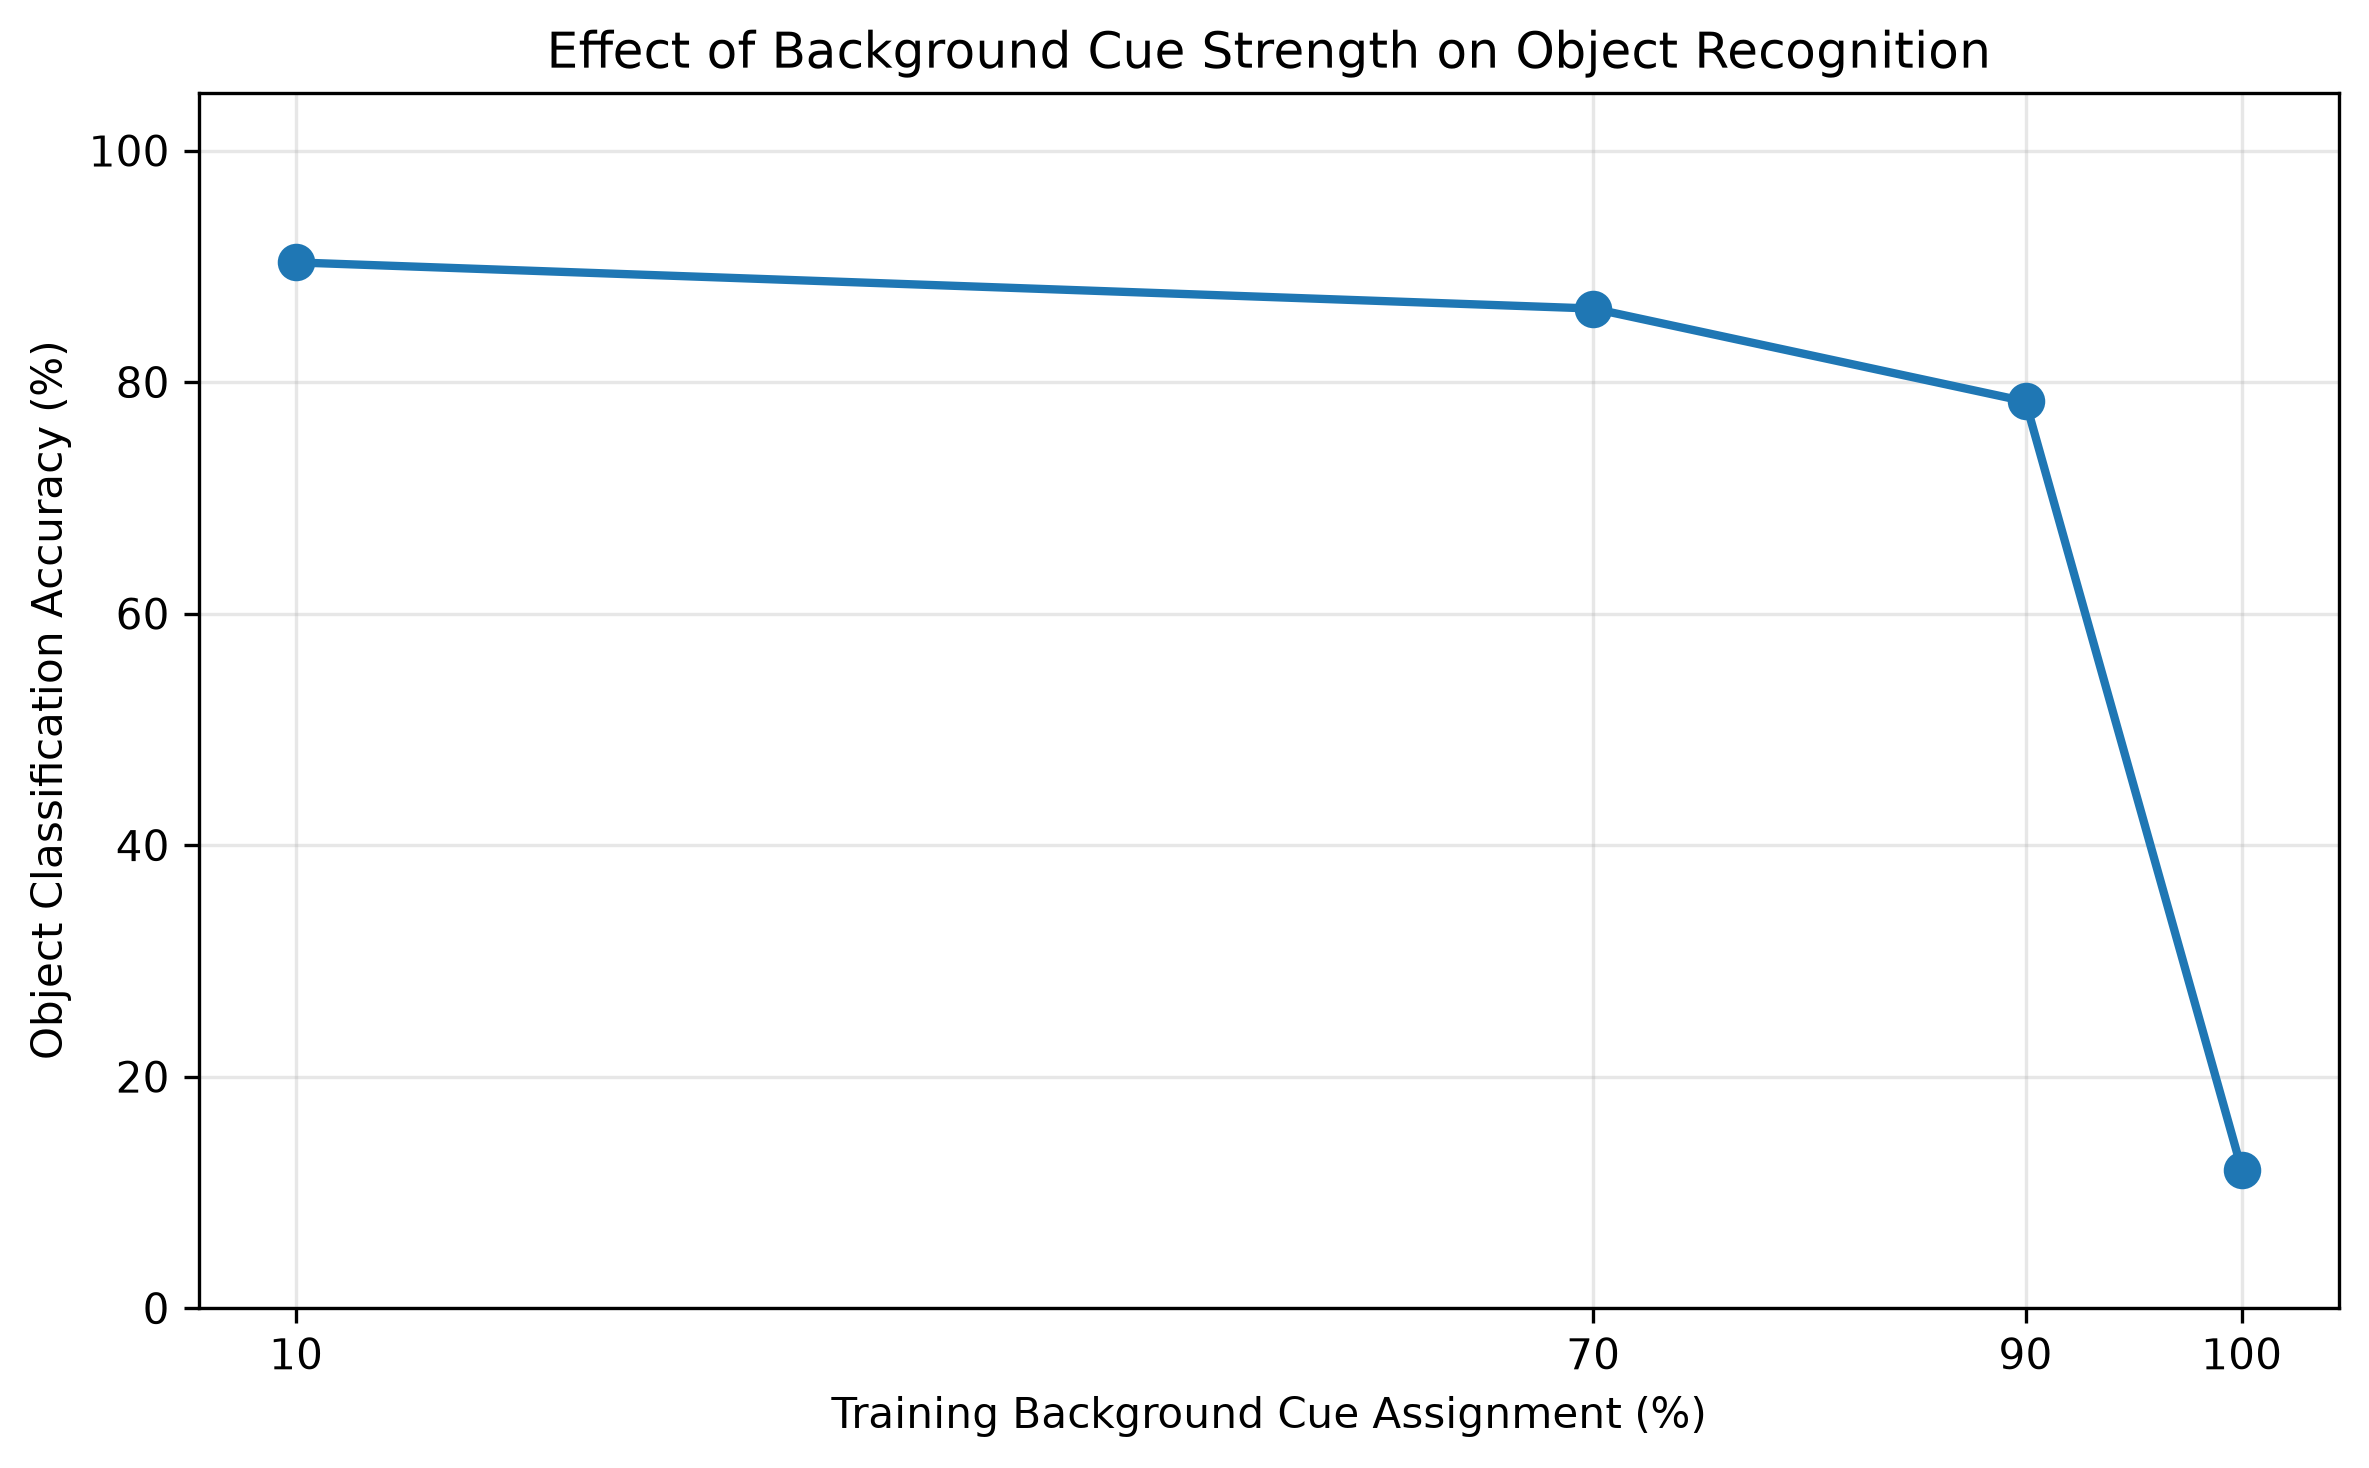
\includegraphics[width=\columnwidth]{figure_1_object_accuracy.png}
\caption{Background model object accuracy under controlled intervention.}
\label{fig:bgacc}
\end{figure}

\begin{figure}[t]
\centering
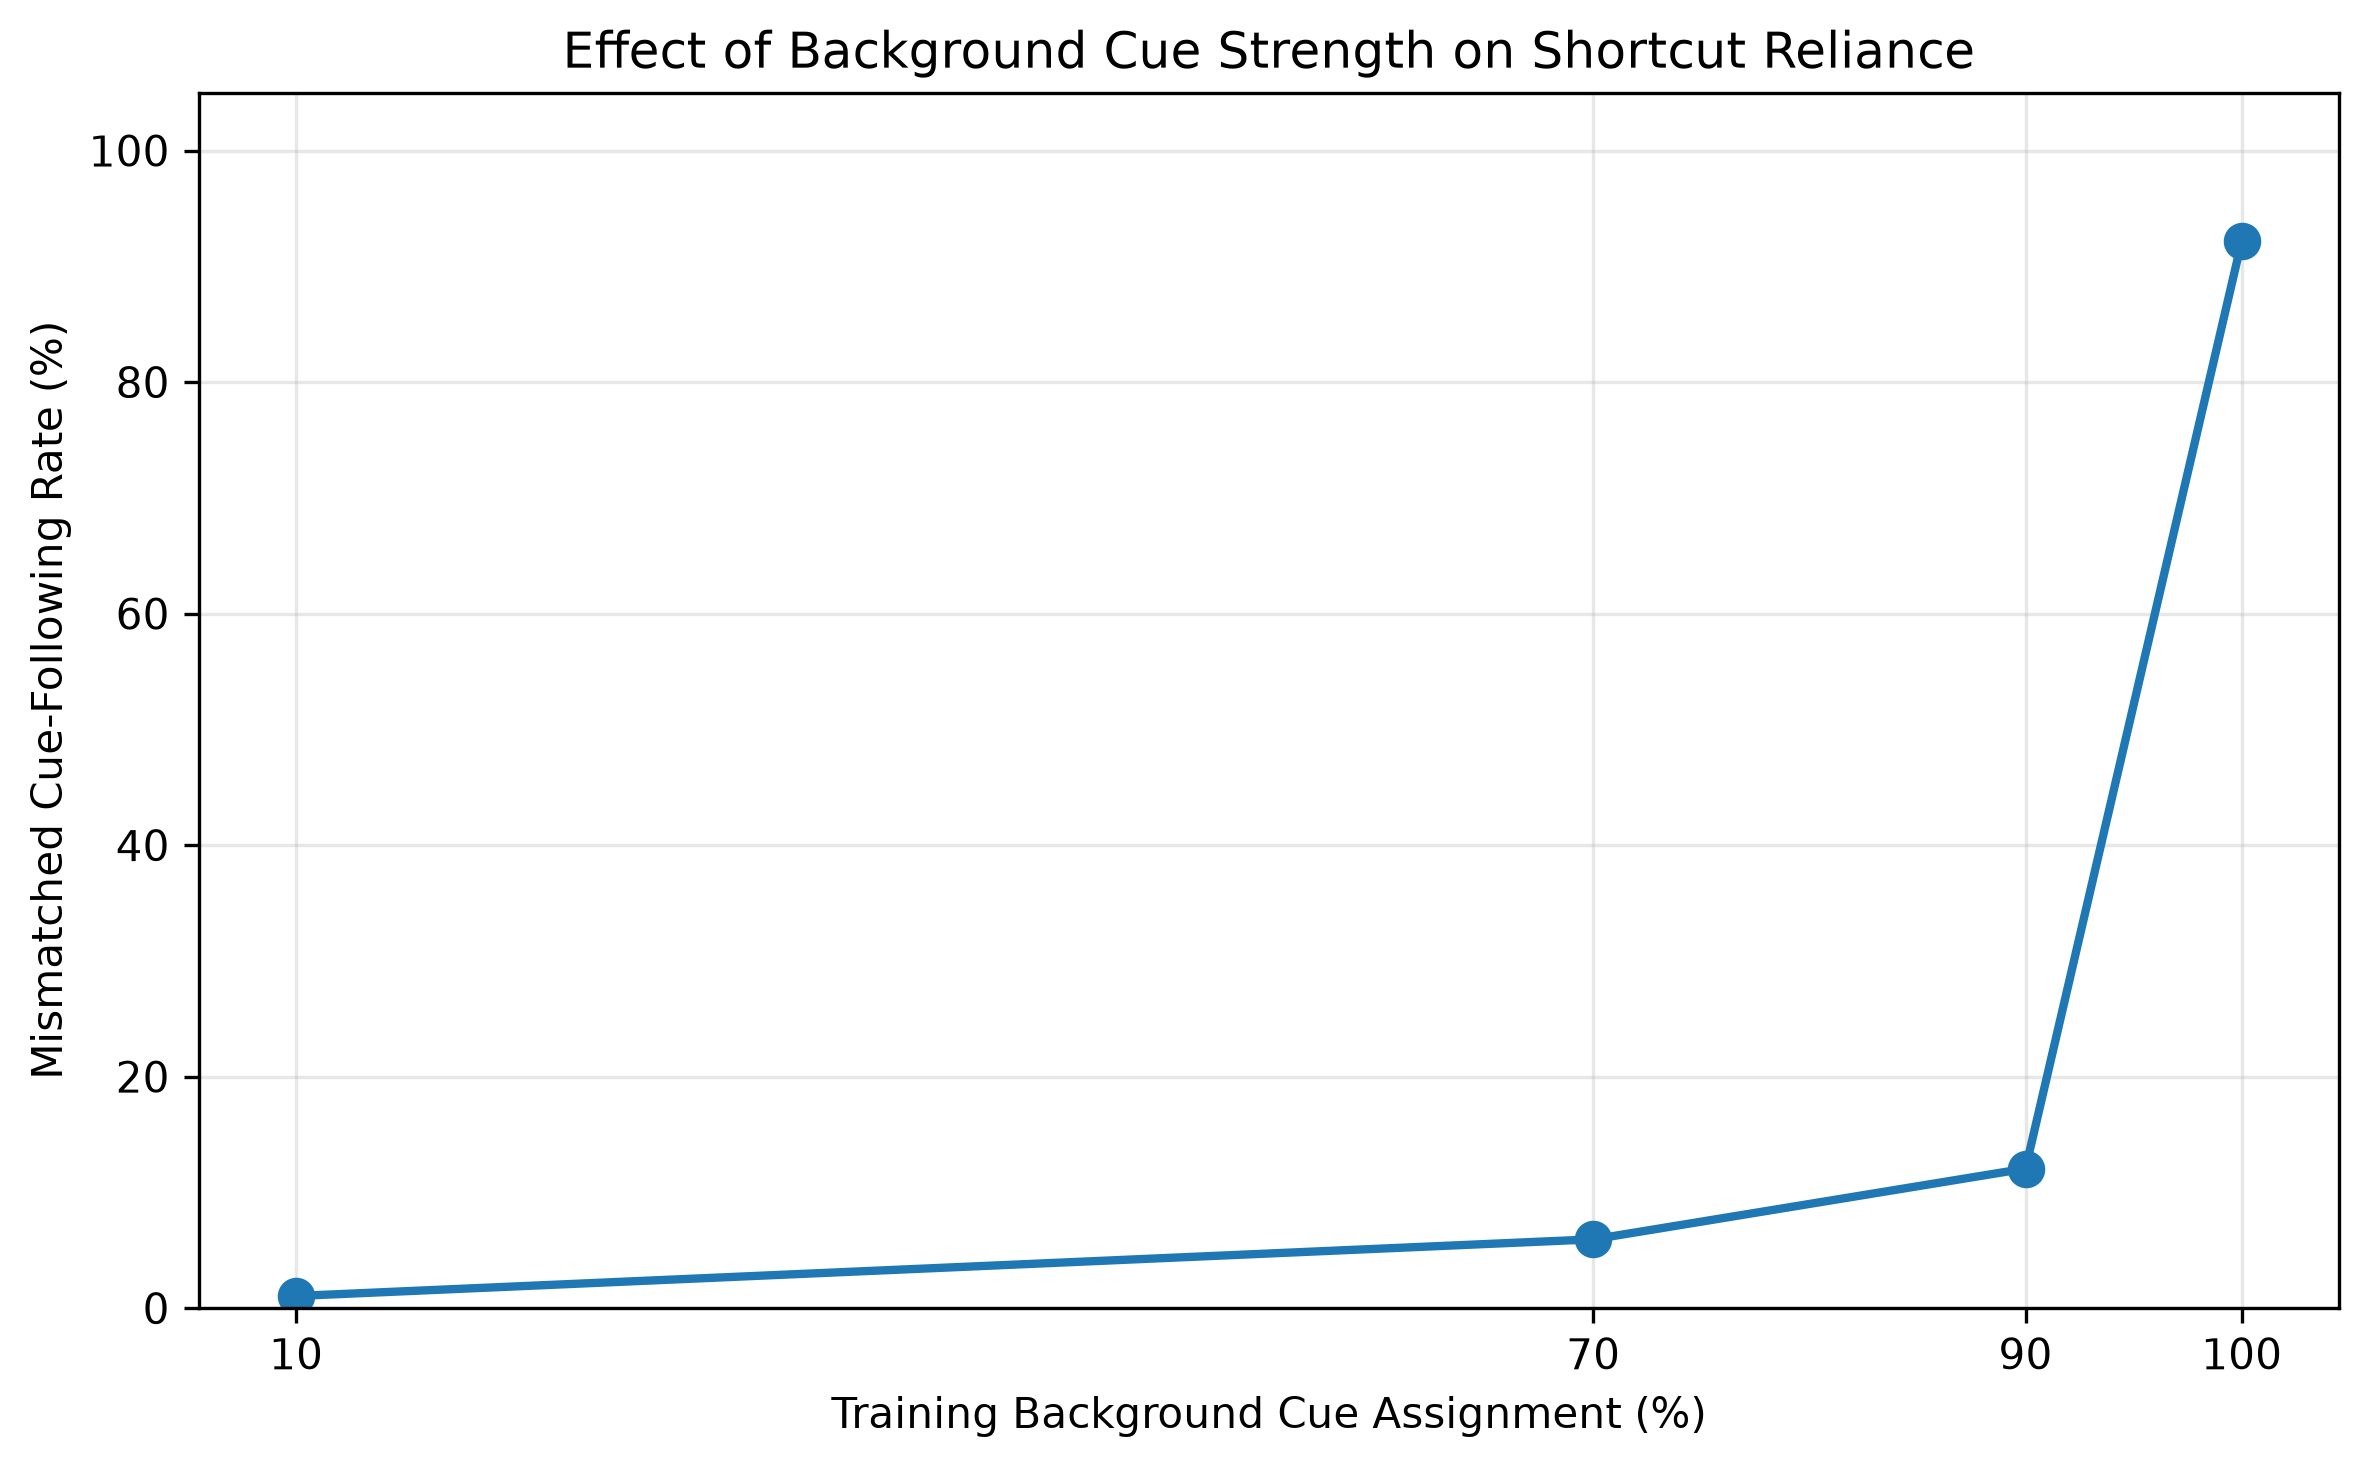
\includegraphics[width=\columnwidth]{figure_2_cue_following.png}
\caption{Background model cue-following under controlled intervention.}
\label{fig:bgcue}
\end{figure}

\begin{figure}[t]
\centering
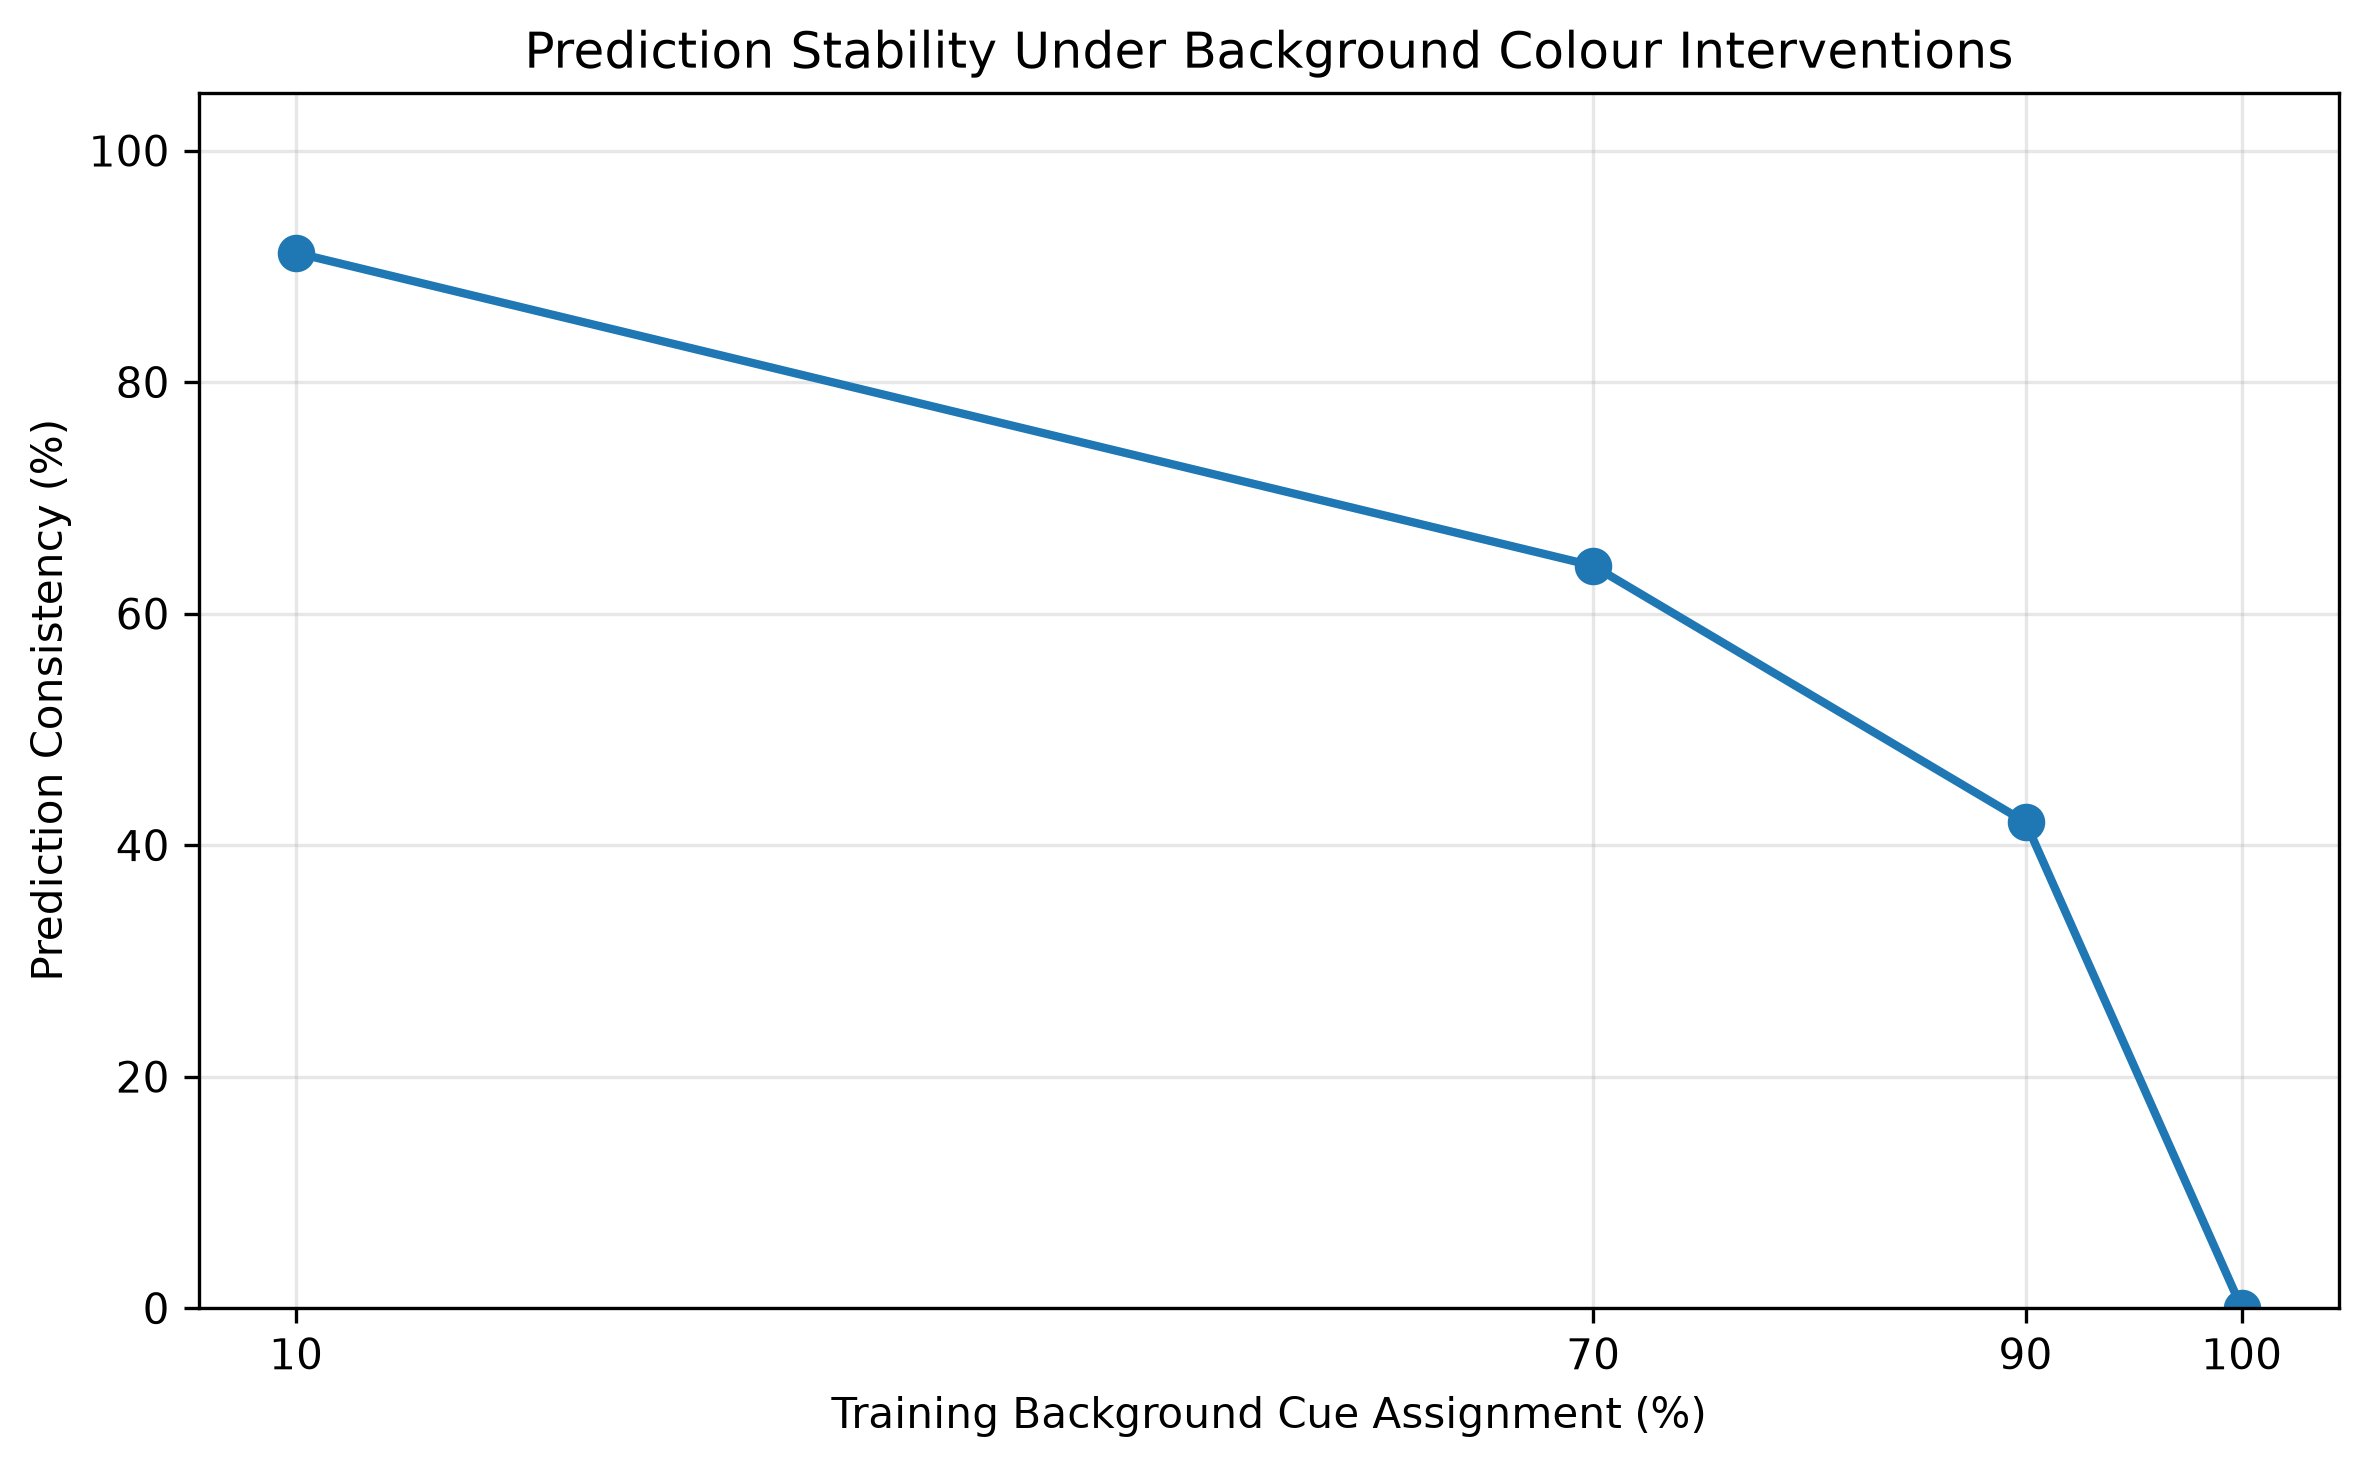
\includegraphics[width=\columnwidth]{figure_3_prediction_consistency.png}
\caption{Background model prediction consistency across cue colours.}
\label{fig:bgcons}
\end{figure}

\begin{figure}[t]
\centering
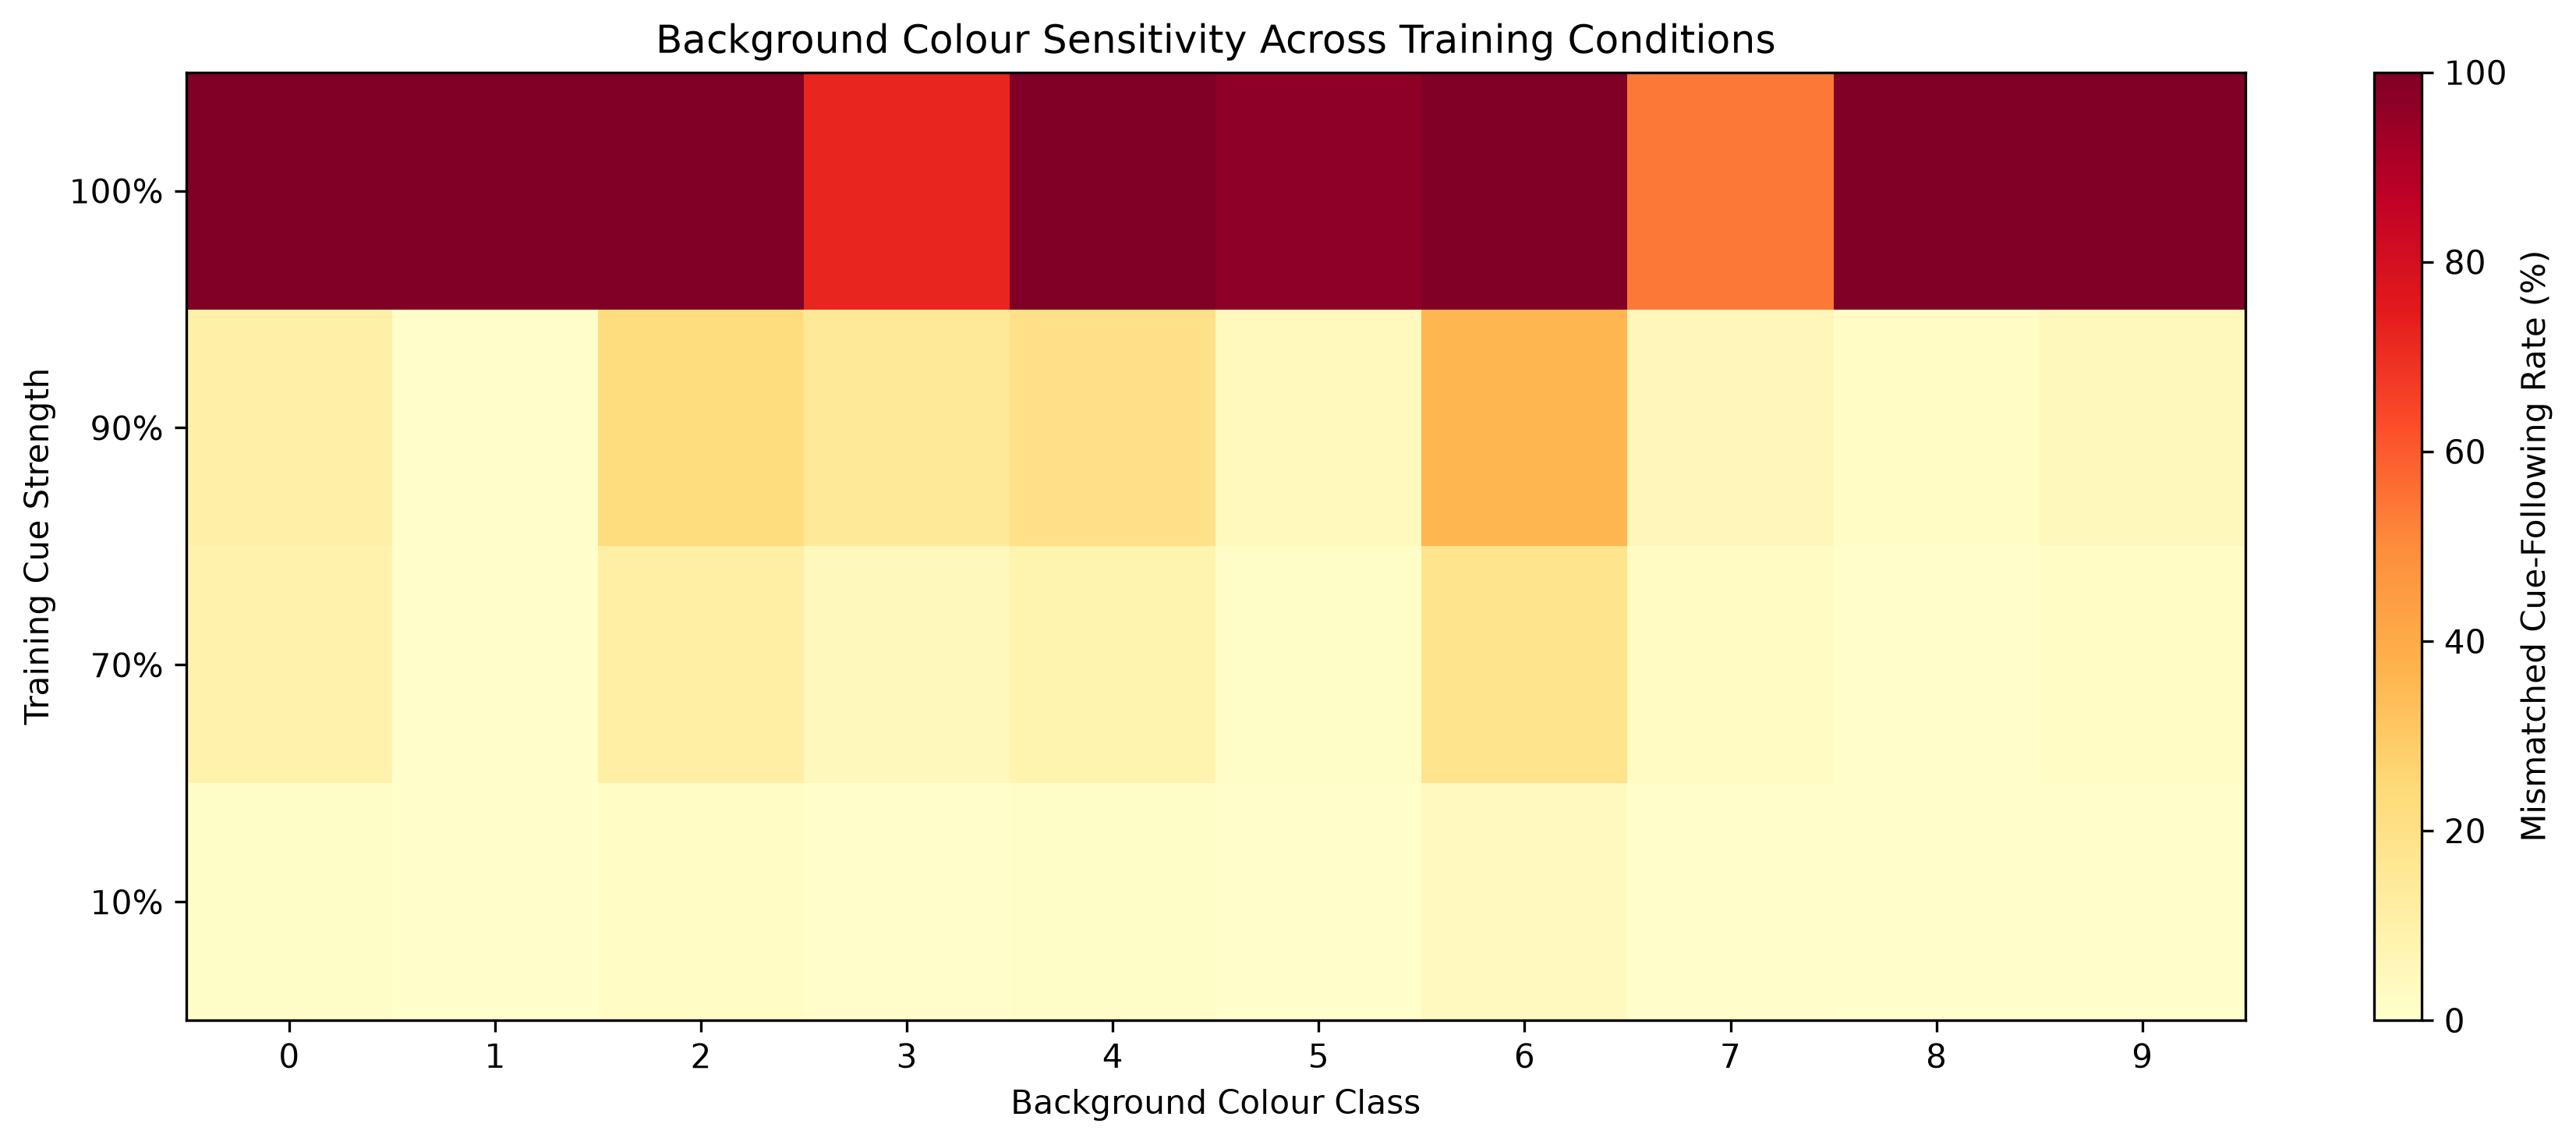
\includegraphics[width=\columnwidth]{figure_4_colour_heatmap.png}
\caption{Per-colour mismatched cue-following rates for the background intervention.}
\label{fig:heatmap}
\end{figure}

\begin{figure}[t]
\centering
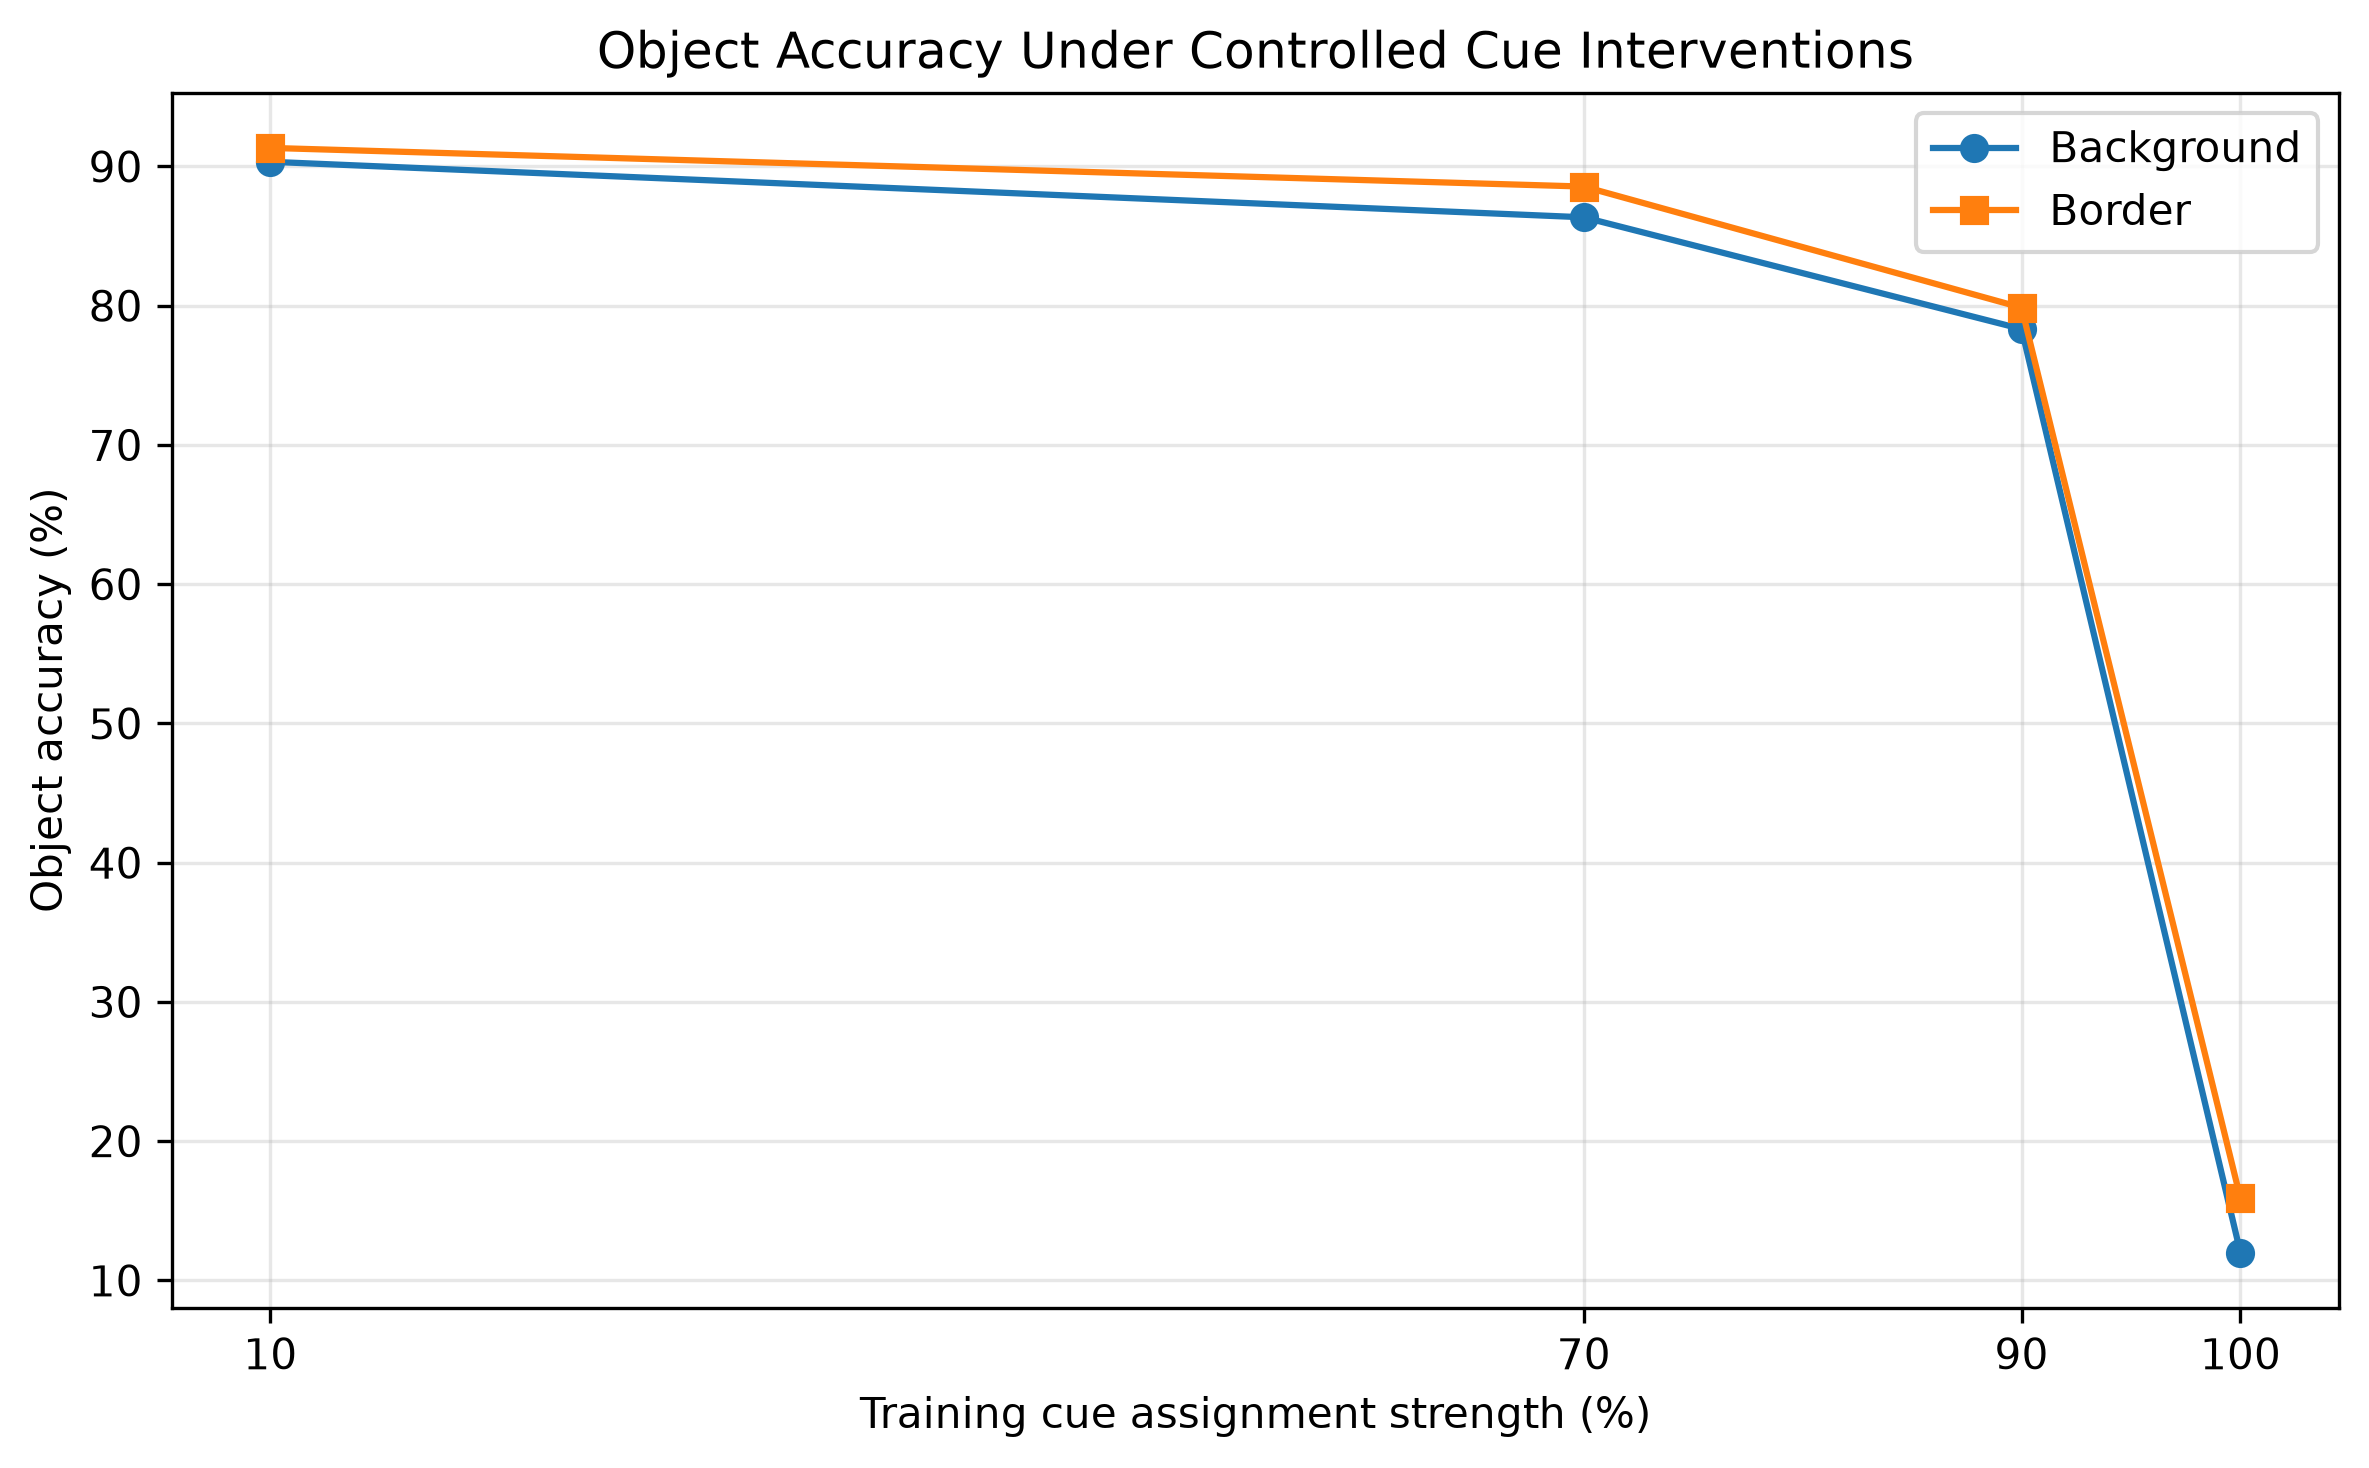
\includegraphics[width=\columnwidth]{figure_5_shortcut_accuracy_comparison.png}
\caption{Object accuracy comparison between background and border interventions.}
\label{fig:compareacc}
\end{figure}

\begin{figure}[t]
\centering
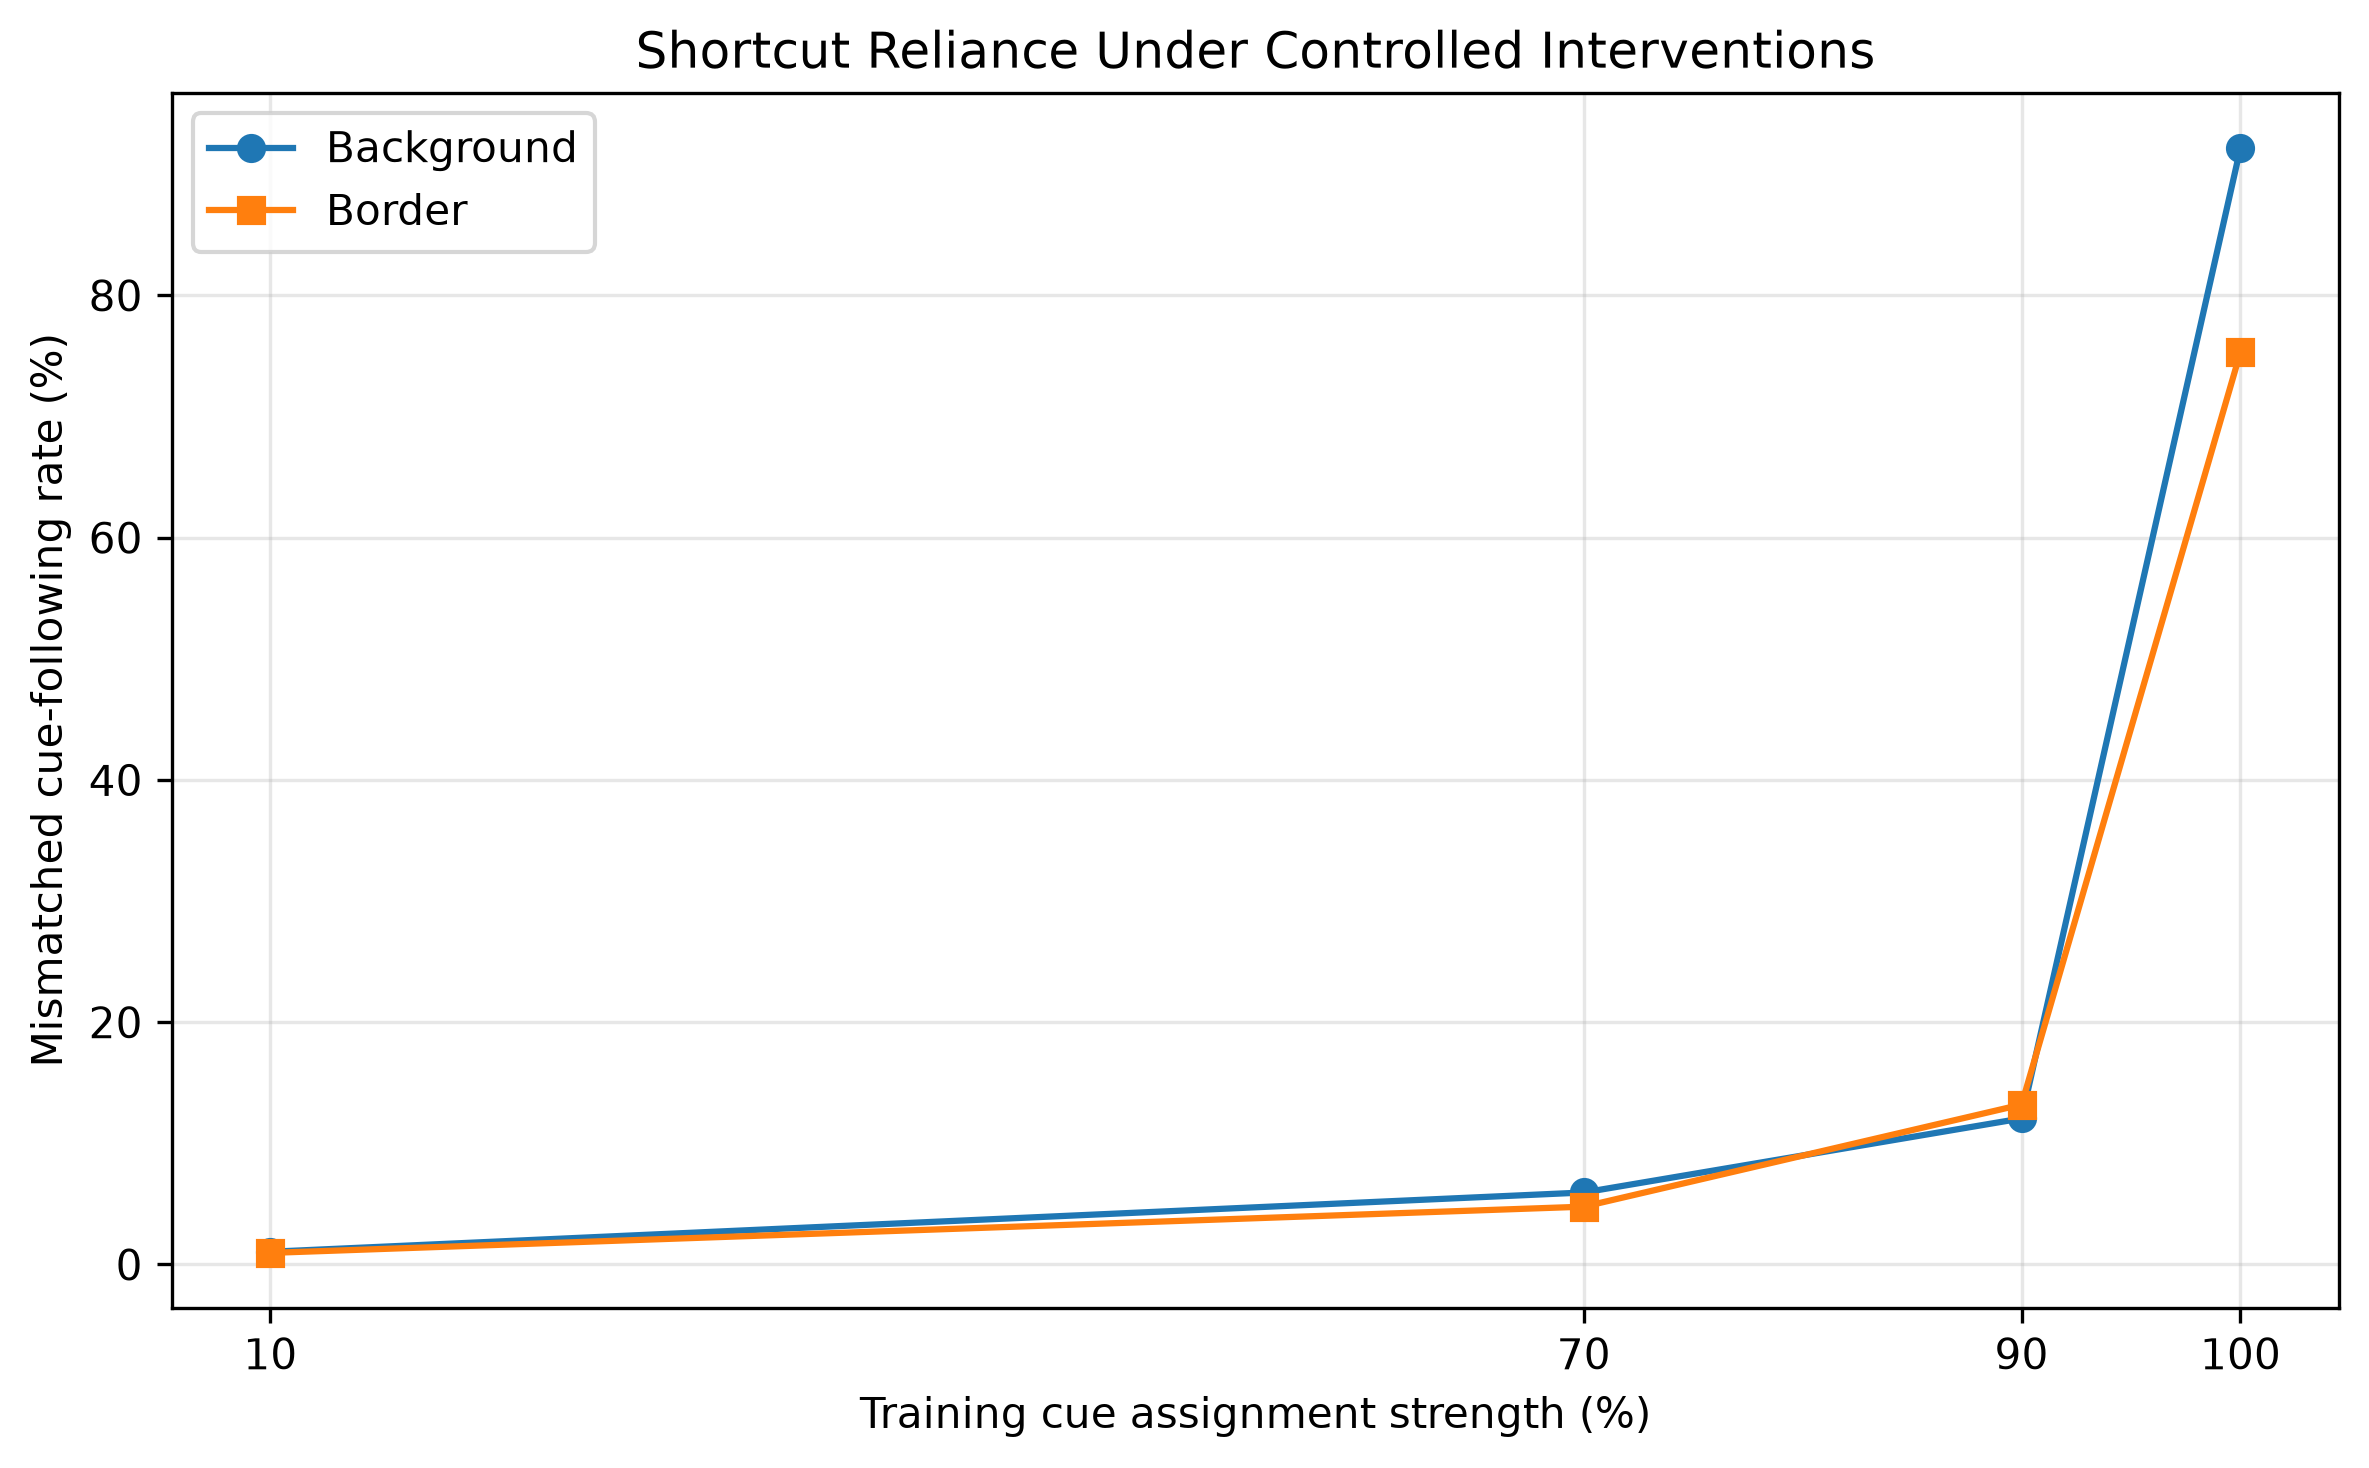
\includegraphics[width=\columnwidth]{figure_6_cue_following_comparison.png}
\caption{Mismatched cue-following comparison between shortcut types.}
\label{fig:comparecue}
\end{figure}

\begin{figure}[t]
\centering
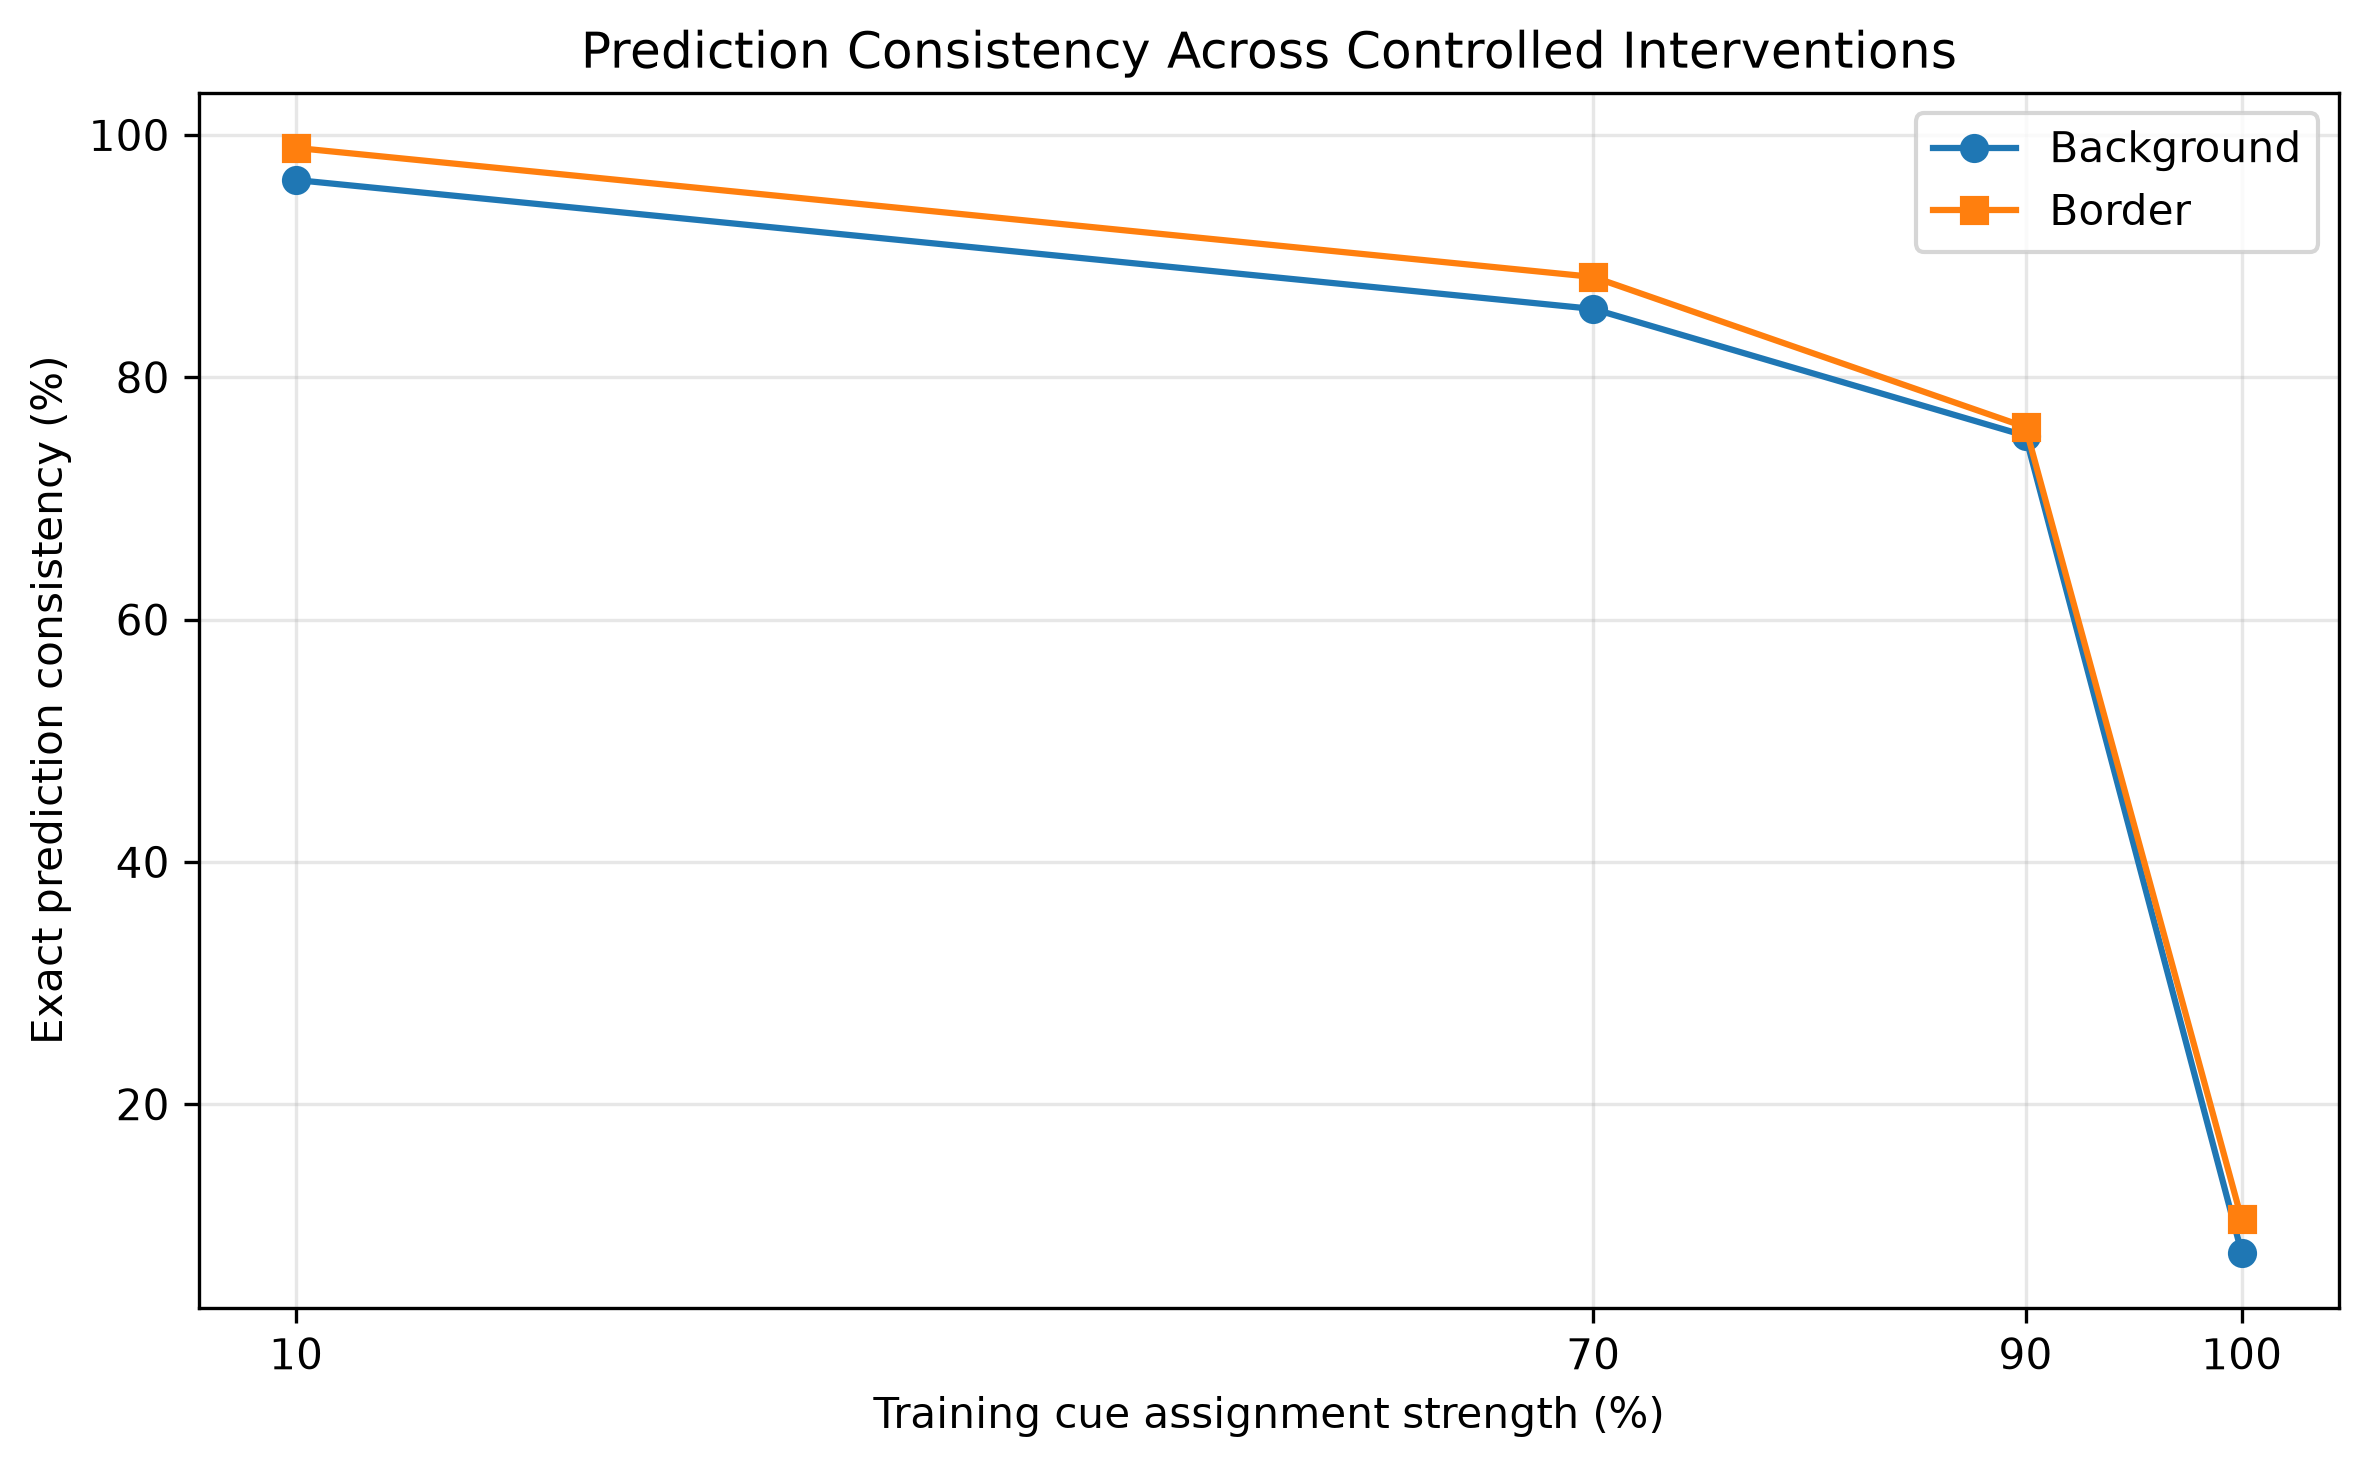
\includegraphics[width=\columnwidth]{figure_7_prediction_consistency_comparison.png}
\caption{Exact prediction consistency comparison between shortcut types.}
\label{fig:comparecons}
\end{figure}

\section{Discussion}
The experiments show that high matched-condition accuracy does not necessarily imply that a classifier bases its decisions on the clothing item. Models trained with 100\% cue assignment achieved near-perfect accuracy when the test cue association was unchanged, but their accuracy and predictions deteriorated sharply when the cue was manipulated. This is consistent with the shortcut-learning behaviour described by Geirhos \emph{et al.} \cite{geirhos}. The controlled interventions strengthen this interpretation because they hold each original image and label fixed while changing only the synthetic cue.

The results also show a graded relationship: models trained with weaker cue-label assignment generally exhibited higher object accuracy and prediction consistency under cue manipulation. At 10\%, the observed cue assignment is approximately uninformative under the balanced class construction, and both model types retained around 90--91\% object accuracy in the intervention. This does not prove that the models use exclusively object-based features, but it indicates much lower dependence on the manipulated cue.

The background and border results are broadly similar in trend, but their numerical differences should not be interpreted as an intrinsic ranking of shortcut types. The input sizes differ ($28\times28$ versus $32\times32$), as do parameter counts. In addition, the background mask replaces all pixels below an intensity threshold and can therefore modify dark clothing regions, whereas the border intervention leaves the original image region unchanged. These design differences confound a direct comparison. The per-colour results also show non-uniform responses: some colours induce substantially more cue-following than others, which may reflect interactions between colour values, learned filters, and class appearance. The present experiment does not isolate the cause of these colour-specific effects.

Several limitations should be considered. Only one training run was conducted per condition, so the results do not provide estimates of run-to-run variability or statistical significance. The experiments use one dataset, one compact CNN family, and synthetic cues; they do not establish how other architectures or natural-image tasks will behave. The low-intensity mask is not a semantic segmentation mask. Finally, cue assignment strength is a controlled probability of assigning the correct class colour, not a direct measurement of statistical correlation in the learned feature representation.

Future work should repeat training across multiple random seeds, match input geometry and parameter counts across shortcut types, and use semantic foreground masks to isolate background pixels more precisely. Additional tests could examine alternative architectures, cue shapes, colour palettes, and naturally occurring spurious features. Such extensions would help determine how broadly the observed behaviour generalises.

\section{Conclusion}
This study investigated synthetic background and border shortcuts in Fashion-MNIST using four cue-assignment strengths and two evaluation protocols. Models trained with perfectly class-correlated cues achieved 99.99\% matched-condition accuracy but showed severe degradation when cue associations changed. Controlled interventions confirmed that predictions could be strongly redirected by changing the cue while preserving the original image and label. Weaker cue-label associations were associated with higher object accuracy and prediction stability under intervention. The findings provide a controlled demonstration of shortcut sensitivity in this experimental setting, while architectural and transformation differences limit direct claims about the relative strength of background and border shortcuts.

\section*{Use of AI Tools}
Generative AI was used as an assistance tool during preparation of this manuscript, including support with language editing, organisation of the paper, and explanation of experimental results. The experimental design decisions, code execution, model training, data generation, evaluation, numerical results, and final verification of the claims remain the responsibility of the author. AI-generated text and suggestions were reviewed and edited by the author. No AI system was used to generate experimental measurements or fabricate results. This declaration should be adjusted if required by the institution's specific disclosure policy.

\balance
\begin{thebibliography}{3}

\bibitem{geirhos}
R. Geirhos, J.-H. Jacobsen, C. Michaelis, R. Zemel, W. Brendel, M. Bethge, and F. A. Wichmann, ``Shortcut learning in deep neural networks,'' \emph{Nature Machine Intelligence}, vol. 2, no. 11, pp. 665--673, 2020, doi: 10.1038/s42256-020-00257-z.

\bibitem{luo}
X. Luo, L. Wei, L. Wen, J. Yang, Z. Xu, and Q. Tian, ``Rectifying the shortcut learning of background for few-shot learning,'' in \emph{Advances in Neural Information Processing Systems}, vol. 34, 2021.

\bibitem{bassi}
P. R. A. S. Bassi, S. S. J. Dertkigil, and A. Cavalli, ``Improving deep neural network generalization and robustness to background bias via layer-wise relevance propagation optimization,'' \emph{Nature Communications}, vol. 15, Art. no. 291, 2024, doi: 10.1038/s41467-023-44371-z.

\end{thebibliography}

\end{document}